% Figure 1: Classifier performance
\begin{figure}[htbp]
\centering
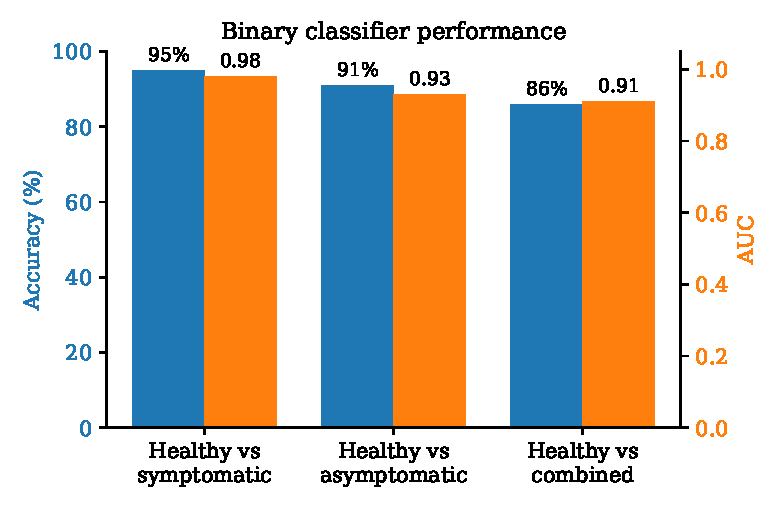
\includegraphics[width=0.75\textwidth]{figures/fig1_classifier.pdf}
\caption{Binary classifier performance for distinguishing healthy donors from
individuals with telomere biology disorders. Using telomere length
measurements and donor age as features, the classifier achieves 95\%
accuracy (AUC $=$ 0.98) for healthy vs.\ symptomatic patients, 91\% accuracy
(AUC $=$ 0.93) for healthy vs.\ asymptomatic carriers, and 86\% accuracy
(AUC $=$ 0.91) for healthy vs.\ the combined TBD group.}
\label{fig:classifier}
\end{figure}

% Figure 2: TERT-null attrition
\begin{figure}[htbp]
\centering
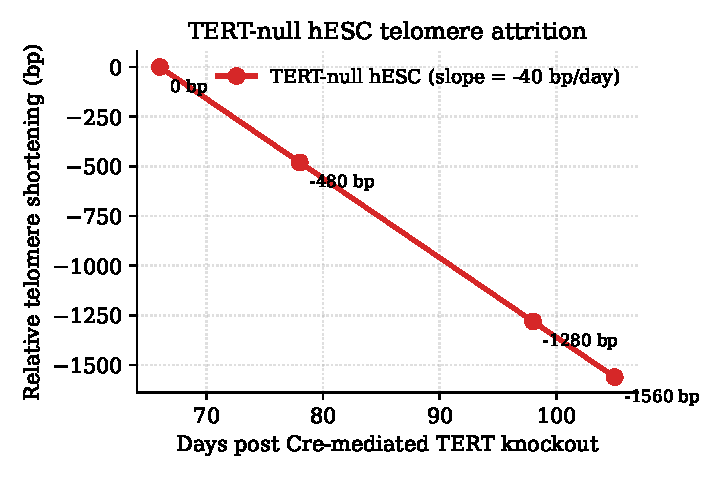
\includegraphics[width=0.65\textwidth]{figures/fig2_tert_attrition.pdf}
\caption{Telomere shortening in TERT-null hESCs. The mean telomere length
decreases linearly across passages sampled at 66, 78, 98, and 105 days
post Cre-mediated TERT inactivation at an average rate of $\sim$40 bp per
day.}
\label{fig:tert}
\end{figure}

% Figure 3: Pipeline schematic
\begin{figure}[htbp]
\centering
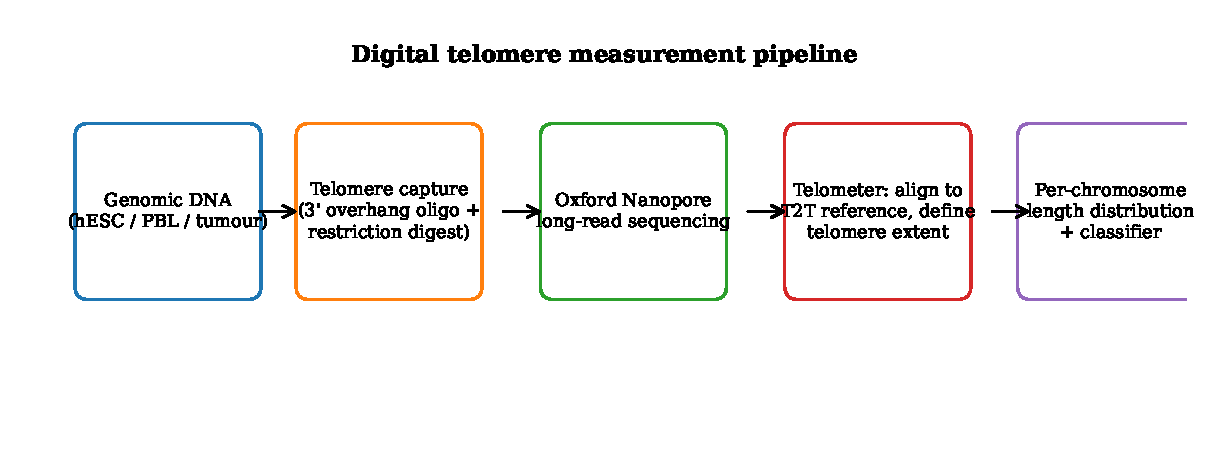
\includegraphics[width=\textwidth]{figures/fig3_schematic.pdf}
\caption{Schematic of the digital telomere measurement pipeline. Genomic
DNA is either subjected to telomere capture (biotinylated oligonucleotide
complementary to the 3$'$ overhang combined with restriction digestion) or
processed as whole-genome input. The sequencing library is run on an
Oxford Nanopore device. Reads are aligned with Telometer to chromosomal
termini of the telomere-to-telomere (T2T) human reference. Per-read
telomere lengths are then aggregated into per-chromosome distributions
and fed to the binary classifier.}
\label{fig:schematic}
\end{figure}

% Figure 4: Aging slopes
\begin{figure}[htbp]
\centering
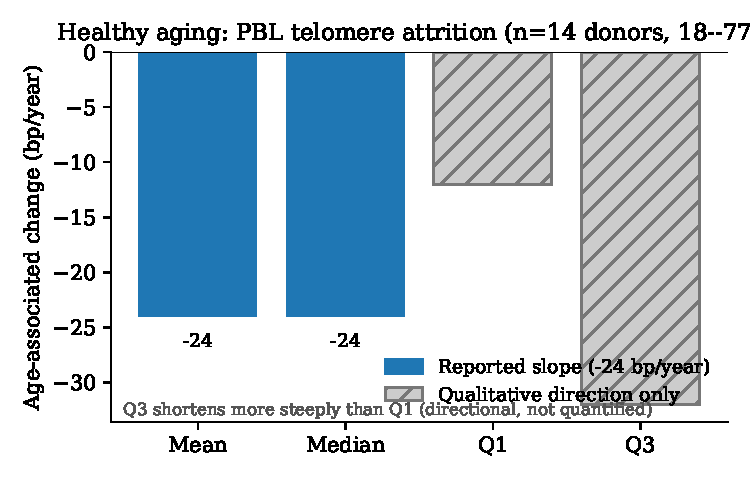
\includegraphics[width=0.7\textwidth]{figures/fig4_aging_slopes.pdf}
\caption{Age-associated telomere attrition in PBLs from 14 healthy donors
(ages 18--77). Mean and median telomere lengths decline by approximately
24 bp/year. The third quartile declines more steeply than the first
quartile, though the quartile-specific slopes are reported only
qualitatively in the underlying data.}
\label{fig:aging}
\end{figure}

% Figure 5: CRC cohort
\begin{figure}[htbp]
\centering
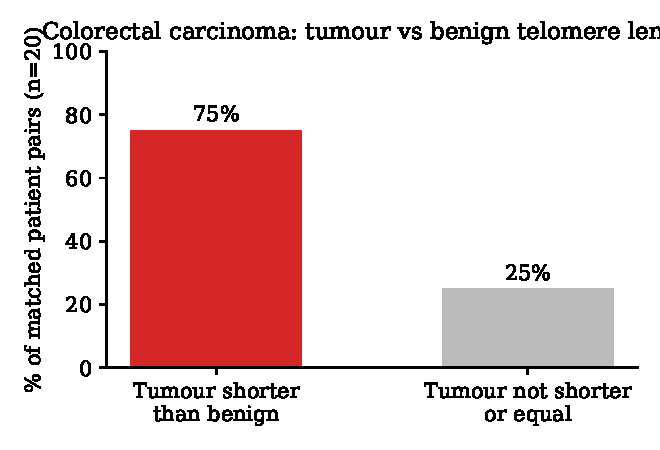
\includegraphics[width=0.6\textwidth]{figures/fig5_crc_tumor_vs_benign.pdf}
\caption{Across 20 patients with matched benign colonic epithelium and
colorectal carcinoma, tumour telomeres are significantly shorter than
benign telomeres in 75\% of patients (Wilcoxon rank-sum test per patient;
30X whole-genome long-read data).}
\label{fig:crc}
\end{figure}
